\subsection{Odległość od optimum}

Z rys. \ref{fig:avg} wynika, że dla każdej instancji problemu, heurystyka i algorytmy przeszukiwania lokalnego osiągają podobne wyniki, które są kilkukrotnie lepsze od rozwiązania losowego, z którego startują zarówno Greedy, jak i Steepest.

\begin{figure}
\begin{center}
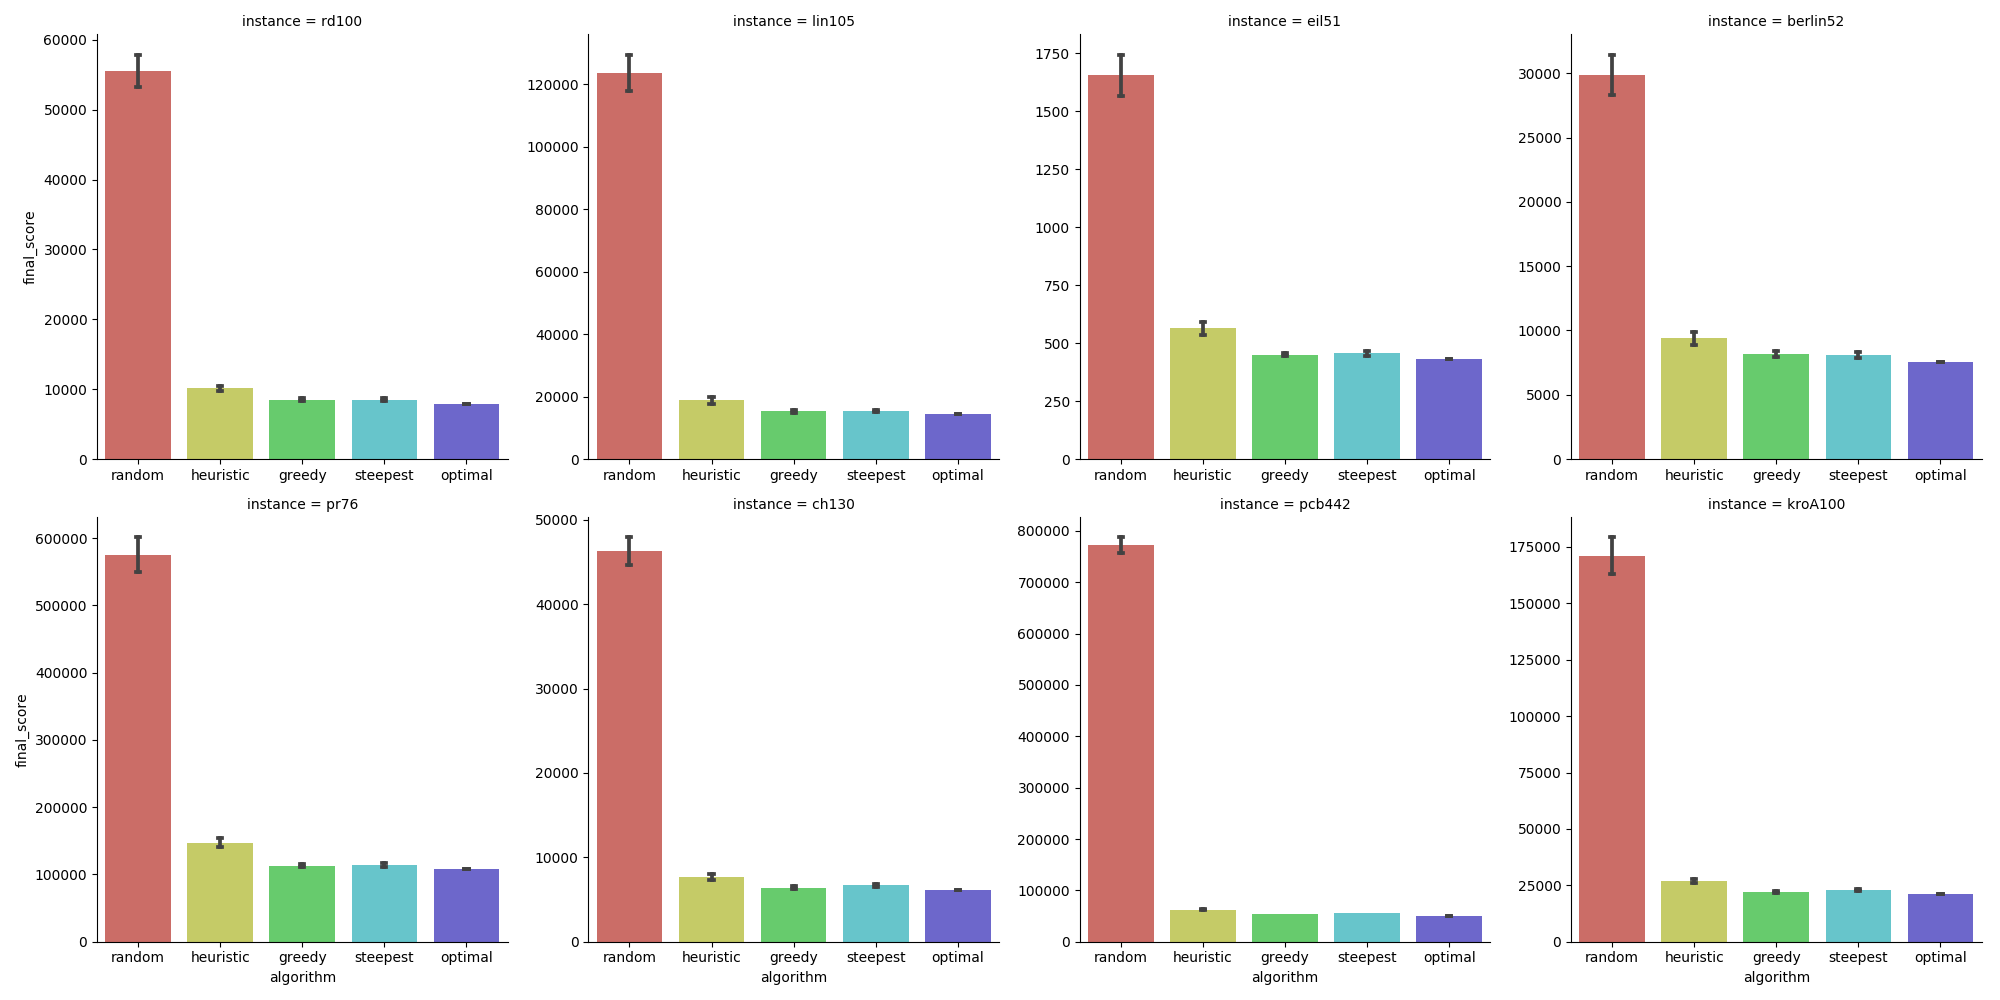
\includegraphics[width=0.8\textwidth]{graphs/algorithm_score_comparison_bar_avg.png}
\end{center}
\caption{Porównanie średnich rozwiązań na~różnych instancjach.}
\label{fig:avg}
\end{figure}

\begin{figure}
\begin{center}
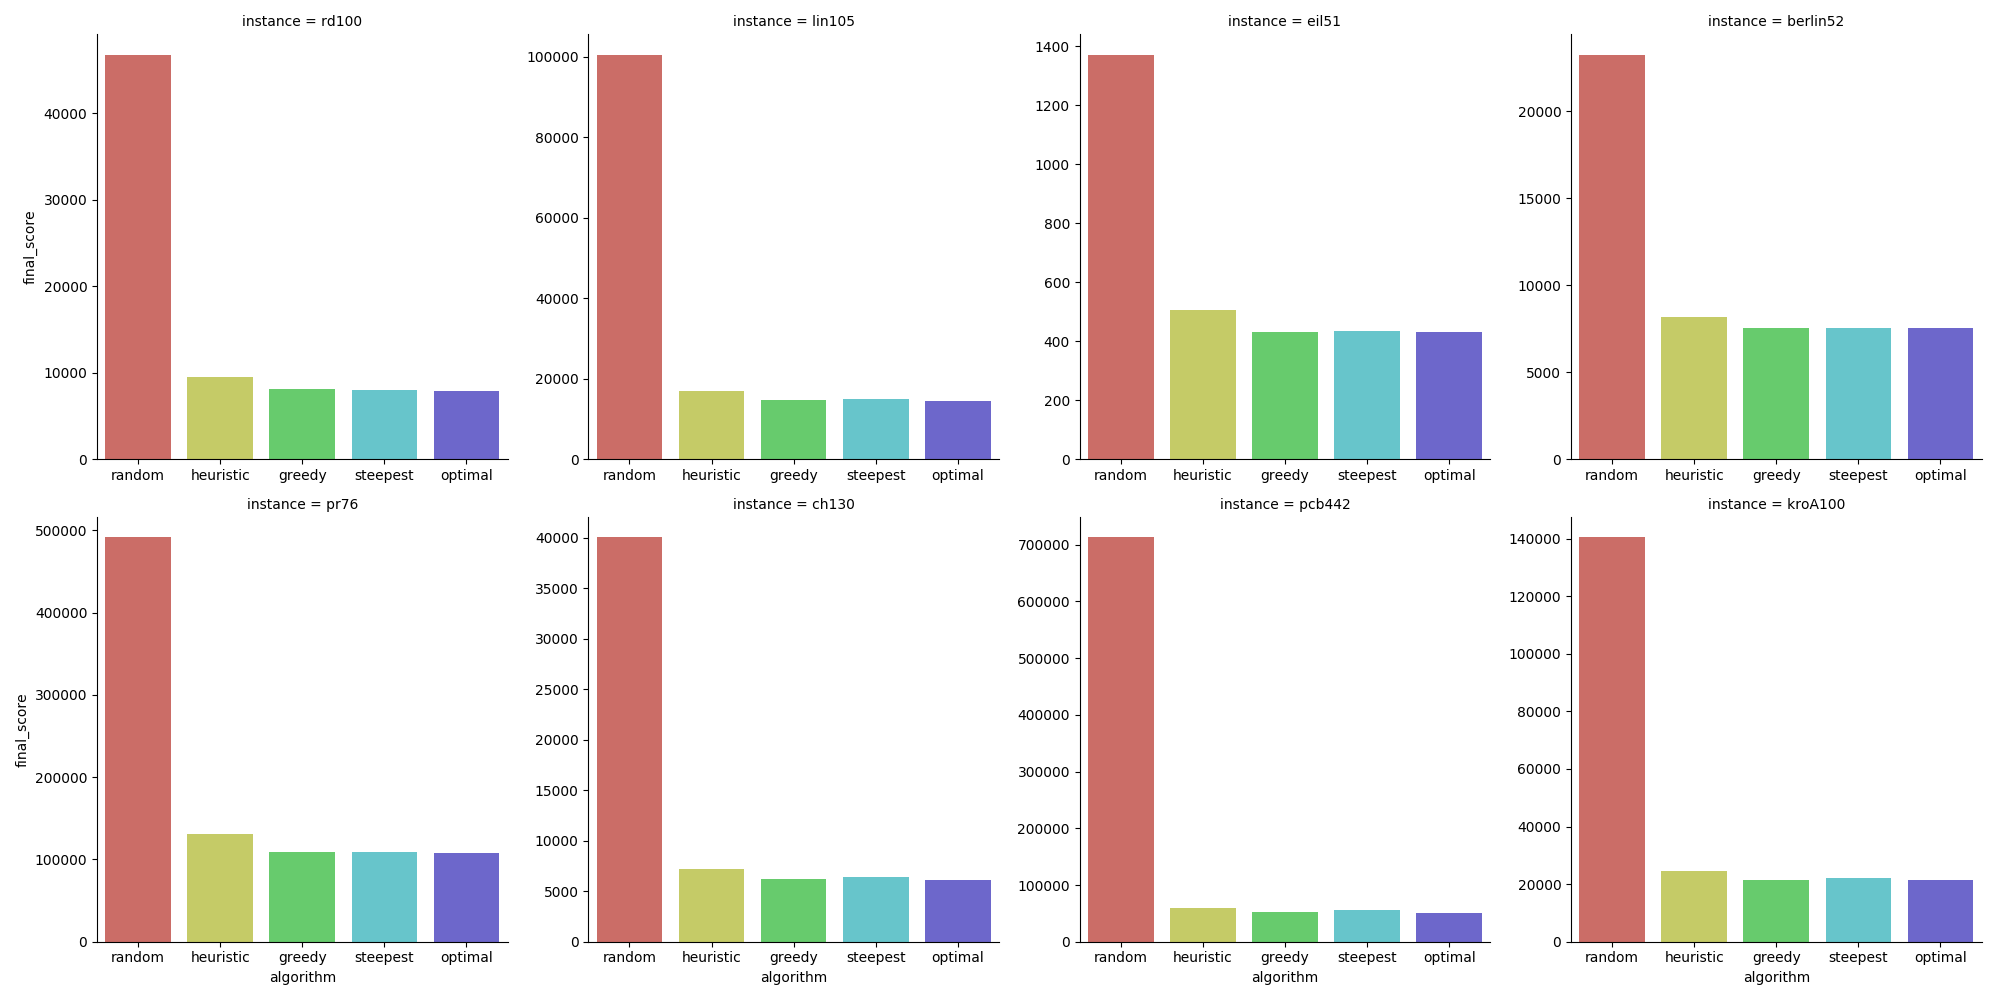
\includegraphics[width=0.8\textwidth]{graphs/algorithm_score_comparison_bar_min.png}
\end{center}
\caption{Porównanie najlepszych znalezionych rozwiązań przez~algorytmy na~różnych instancjach.}
\label{fig:best}
\end{figure}

\begin{figure}
\begin{center}
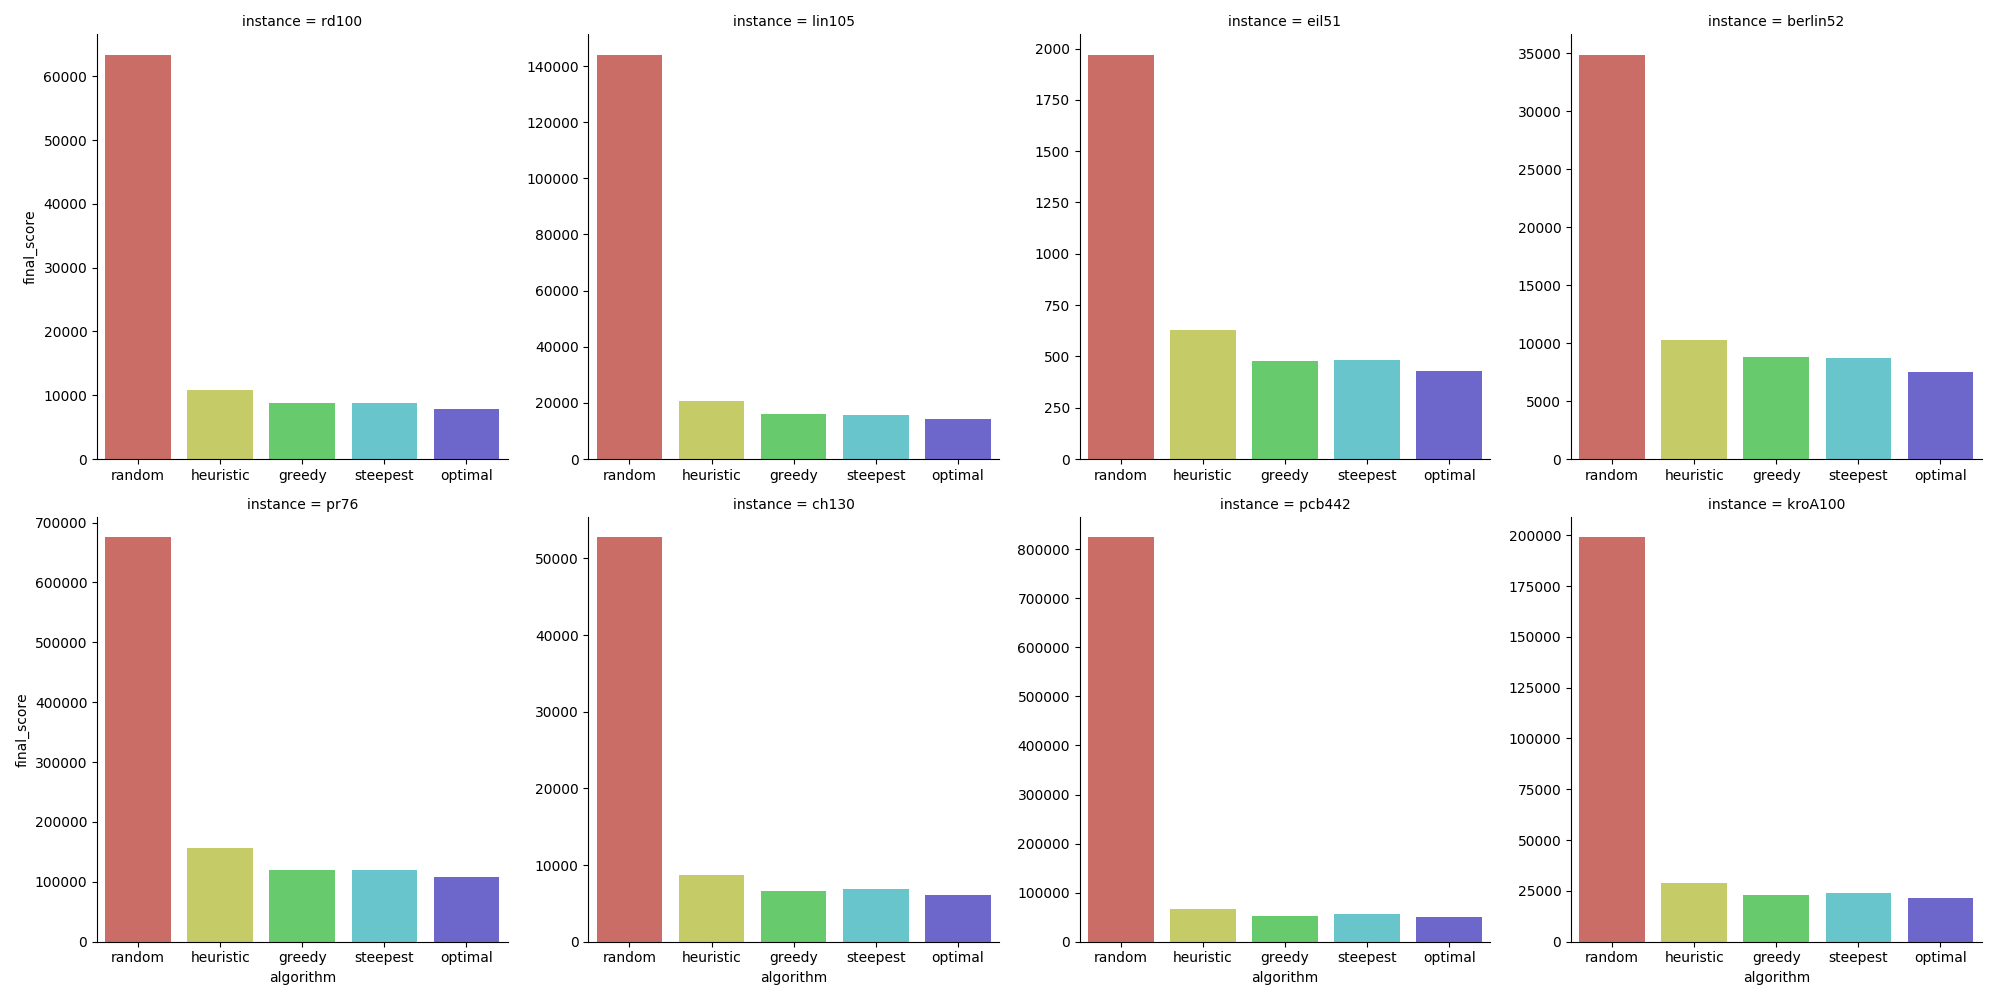
\includegraphics[width=0.8\textwidth]{graphs/algorithm_score_comparison_bar_max.png}
\end{center}
\caption{Porównanie najgorszych znalezionych rozwiązań przez~algorytmy na~różnych instancjach.}
\label{fig:worst}
\end{figure}

\begin{figure}
\begin{center}
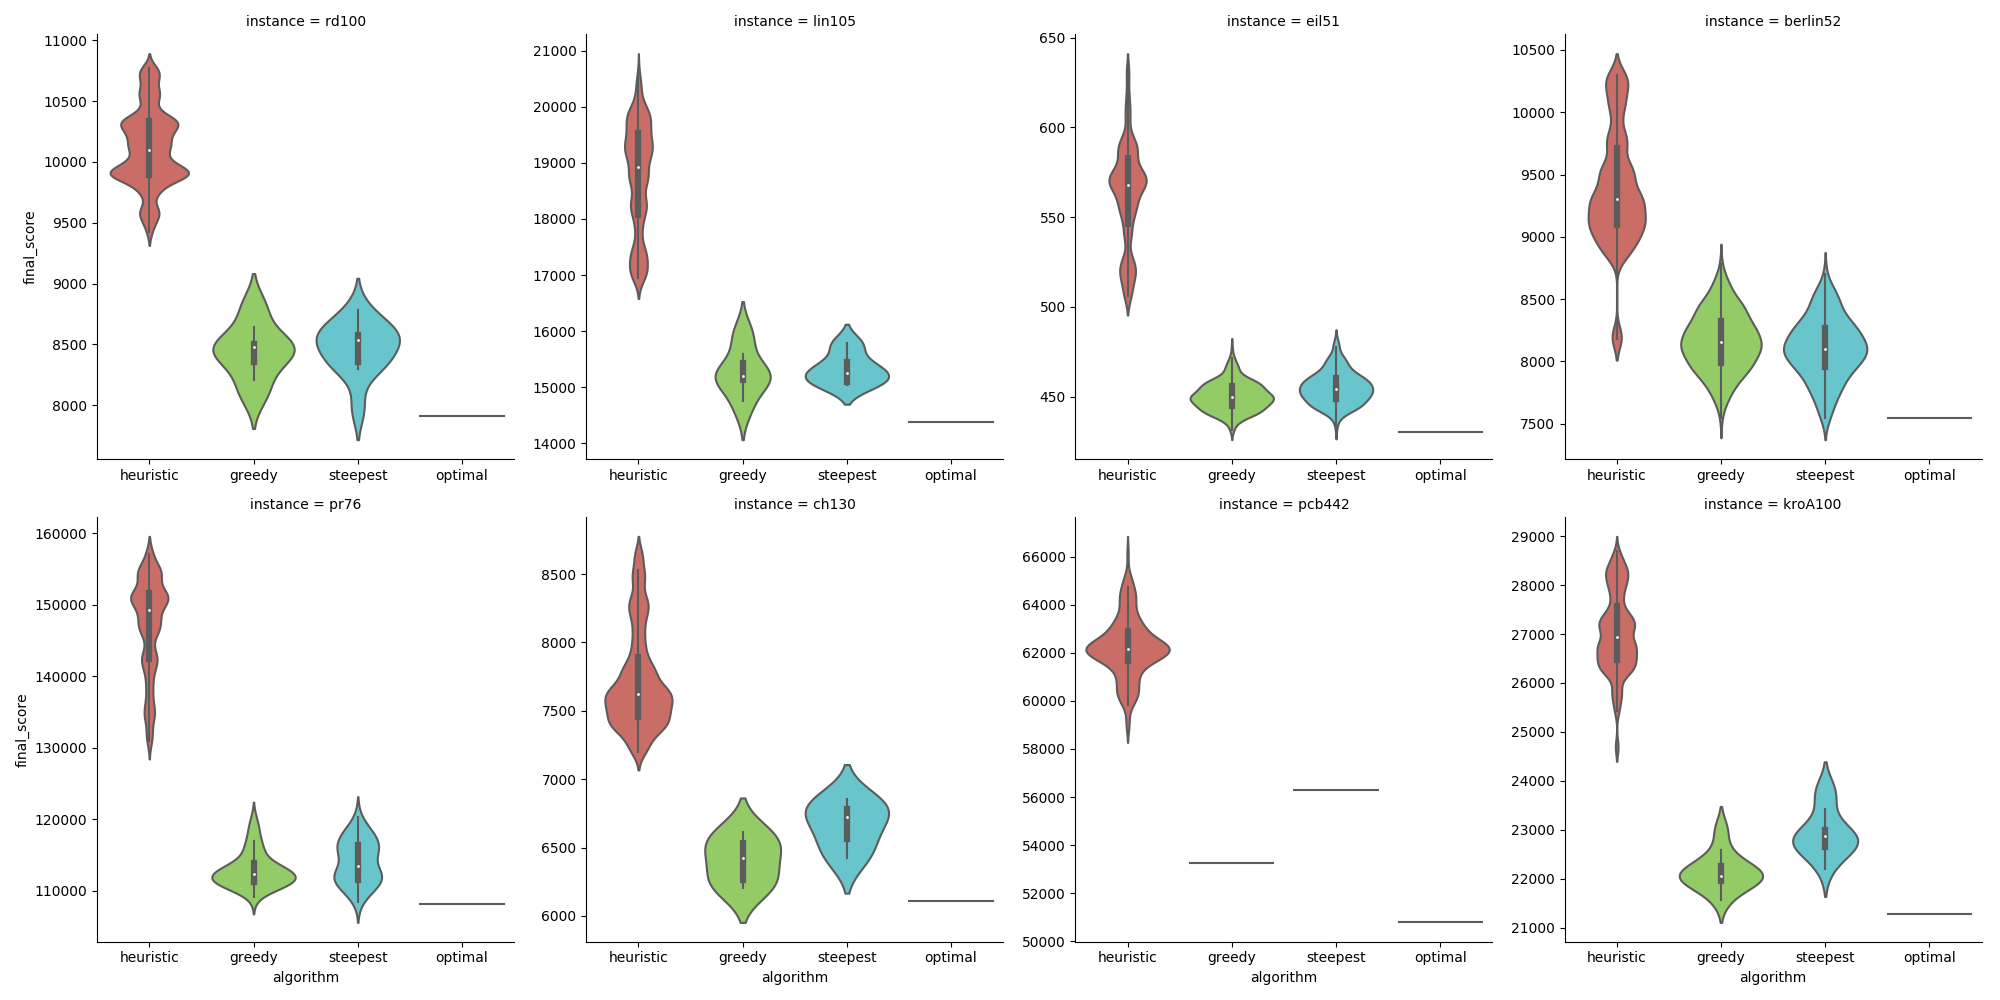
\includegraphics[width=0.8\textwidth]{graphs/algorithm_score_comparison_violin.png}
\end{center}
\caption{Porównanie rozkładów znalezionych rozwiązań przez~algorytmy na~różnych instancjach.}
\label{fig:distribution}
\end{figure}

\subsection{Czas działania}

Algorytm losowy oraz heurystyka są zdecydowanie najszybsze, ponieważ każde z nich sprawdza tylko jedno rozwiązanie. Greedy i Steepest przeszukują przestrzeń rozwiązań, dopóki nie mogą już bardziej poprawić wyniku, co zajmuje znacznie więcej czasu.

\begin{figure}
\begin{center}
%\includegraphics[width=0.8\textwidth]{graphs/rys_time.pdf}
\end{center}
\caption{Porównanie czasu działania algorytmów na~poszczególnych instancjach.}
\label{fig:best}
\end{figure}

\subsection{Efektywność algorytmów}

\subsubsection{Wybrana miara}

Aby porównać algorytmy pod względem jakości, można to zrobić przez zdefiniowanie kosztu czasowego, jaki trzeba ponieść, aby uzyskać dane rozwiązanie. Czyli należy policzyć iloraz $cost = time / result$, co przedstawia rys. \ref{fig:cost}. Natomiast efektywnością algorytmu jest odwrotność kosztu, która została przedstawiona na rys. \ref{fig:quality}.

\subsubsection{Wyniki}

Z wykresów \ref{fig:cost} i \ref{fig:quality} można by wyciągnąć wniosek, że najefektywniejszym algorytmem są losowy i heurystyka, ponieważ zajmują najmniej czasu. Nie można przy tym jednak zapominać... %TODO

\begin{figure}
\begin{center}
%\includegraphics[width=0.8\textwidth]{graphs/rys_efficiency.pdf}
\end{center}
\caption{Porównanie kosztów algorytmów na~poszczególnych instancjach.}
\label{fig:cost}
\end{figure}

\begin{figure}
\begin{center}
%\includegraphics[width=0.8\textwidth]{graphs/rys_efficiency.pdf}
\end{center}
\caption{Porównanie efektywności algorytmów na~poszczególnych instancjach.}
\label{fig:quality}
\end{figure}

\subsection{Średnia liczba kroków}

...

\begin{figure}
\begin{center}
%\includegraphics[width=0.8\textwidth]{graphs/rys_steps.pdf}
\end{center}
\caption{Porównanie algorytmów Greedy Search i~Steepest pod~względem liczby kroków do~zatrzymania.}
\label{fig:steps}
\end{figure}

\subsection{Średnia liczba przeszukanych rozwiązań}

...

\begin{figure}
\begin{center}
%\includegraphics[width=0.8\textwidth]{graphs/rys_n_solutions.pdf}
\end{center}
\caption{Porównanie algorytmów Greedy Search i~Steepest pod~względem liczby przeszukanych rozwiązań.}
\label{fig:nsol}
\end{figure}

\subsection{Greedy Search}

\subsubsection{Jakość rozwiązania początkowego a końcowego}

...

\begin{figure}
\begin{center}
%\includegraphics[width=0.8\textwidth]{graphs/rys_difference_start_final.pdf}
\end{center}
\caption{Porównanie jakości rozwiązań początkowych i~końcowych przez~algorytmy Greedy Search i~Steepest.}
\label{fig:diff}
\end{figure}

\subsubsection{Wielokrotne uruchamianie dla różnych rozwiązań początkowych}

...

\begin{figure}
\begin{center}
%\includegraphics[width=0.8\textwidth]{graphs/rys_more_starts.pdf}
\end{center}
\caption{Porównanie jakości rozwiązań algorytmów Gready Search i~Steepest w~zależności od~liczby uruchomień tych algorytmów dla~różnych rozwiązań początkowych.}
\label{fig:more}
\end{figure}

\subsection{Porównanie rozwiązań}

\subsubsection{Miara odległości rozwiązań od rozwiązania optymalnego}

...

\subsubsection{Wyniki}

...

\begin{figure}
\begin{center}
%\includegraphics[width=0.8\textwidth]{graphs/rys_opt_distance.pdf}
\end{center}
\caption{Porównanie odległości znajdowanych rozwiązań przez algorytmy od rozwiązania optymalnego.}
\label{fig:dist}
\end{figure}